%%%%%%%%%%%%%%%%%%%%%%%%%%%%%%%%%%%%%%%%%%%%%%%%%%%%%%%%%%%%%%%%%%%%%%%%%%%%%%%%
%2345678901234567890123456789012345678901234567890123456789012345678901234567890
%        1         2         3         4         5         6         7         8

\documentclass[letterpaper, 10 pt, conference]{ieeeconf}  % Comment this line out
                                                          % if you need a4paper
%\documentclass[a4paper, 10pt, conference]{ieeeconf}      % Use this line for a4
                                                          % paper

\IEEEoverridecommandlockouts                              % This command is only
                                                          % needed if you want to
                                                          % use the \thanks command
\overrideIEEEmargins

\usepackage{times}
\usepackage[T1]{fontenc}
\usepackage{tikz}
\usepackage{amsmath}
%\usepackage{amsthm}
%\usepackage{verbatim}
\usepackage{subfigure}
\usepackage{graphicx}
\usepackage{wrapfig}

\newcommand{\comments}[1]{}
% See the \addtolength command later in the file to balance the column lengths
% on the last page of the document



% The following packages can be found on http:\\www.ctan.org
\usepackage{graphics} % for pdf, bitmapped graphics files
\usepackage{epsfig} % for postscript graphics files
\usepackage{mathptmx} % assumes new font selection scheme installed
\usepackage{times} % assumes new font selection scheme installed
\usepackage{amsmath} % assumes amsmath package installed
\usepackage{amssymb}  % assumes amsmath package installed

\usepackage{amsmath}
\interdisplaylinepenalty=2500

\title{\LARGE \bf
The Conjugate Unscented Transform
}
\comments{
\author{ \parbox{3 in}{\centering Huibert Kwakernaak*
         \thanks{*Use the $\backslash$thanks command to put information here}\\
         Faculty of Electrical Engineering, Mathematics and Computer Science\\
         University of Twente\\
         7500 AE Enschede, The Netherlands\\
         {\tt\small h.kwakernaak@autsubmit.com}}
         \hspace*{ 0.5 in}
         \parbox{3 in}{ \centering Pradeep Misra**
         \thanks{**The footnote marks may be inserted manually}\\
        Department of Electrical Engineering \\
         Wright State University\\
         Dayton, OH 45435, USA\\
         {\tt\small pmisra@cs.wright.edu}}
}
}
\author{\begin{tabular}{cccc}
 Nagavenkat Adurthi  &  Puneet Singla &  Tarunraj Singh \\
Graduate Student & Assistant Professor & Professor \\
nagavenk@buffalo.edu & psingla@buffalo.edu & tsingh@buffalo.edu \vspace{0.01in}\end{tabular}\\
%\textsl{Department of Mechanical \& Aerospace Engineering}\\
\textsl{University at Buffalo, State University of New York,
Amherst, NY 14260-4400}}

\begin{document}



\maketitle
\thispagestyle{empty}
\pagestyle{empty}


%%%%%%%%%%%%%%%%%%%%%%%%%%%%%%%%%%%%%%%%%%%%%%%%%%%%%%%%%%%%%%%%%%%%%%%%%%%%%%%%
\begin{abstract}
This paper presents a scheme to evaluate fully symmetric sigma points with positive weights for the Unscented Transform that can capture higher order moments. This work can be considered as an extension to the $2n+1$ Unscented Transform rule. Besides its application in filtering, it can be used as a Gaussian Cubature rule with reduced number of cubature points compared to the Gauss Hermite product rule. A general Gaussian Cubature rule, applicable to any dimension, is developed that is accurate for polynomials of degree 5 or less. Further, the method is extended till 6th dimension that is accurate for polynomials of degree 9 or less. Results for various non-polynomial type functions are also shown that encourage the develoment of higher order cubature rules with reduced number of points.      
\end{abstract}


%%%%%%%%%%%%%%%%%%%%%%%%%%%%%%%%%%%%%%%%%%%%%%%%%%%%%%%%%%%%%%%%%%%%%%%%%%%%%%%%
\section{INTRODUCTION}
The motivation to carry out the analysis presented in the paper is based on the fact that, "`The more moments the sigma point set capture, the more is the integral value close to the true value"'. To elaborate, when more sigma points are evaluated such that they can satisfy the higher order moment constraint equations (\ref{momentconst}), the integral vaule evaluated by (\ref{sigmasum}) tends to converge to the 'true' value of the integral. By 'true' value we mean the analytical answer if it is available or the \emph{converged} numerical value evaluated by the Gauss-Hermite product rule. The word \emph{converged} is stressed because for a non-polynomial function one usually does not know the adequate number of points for convergence. But it is well known that for a polynomial of degree $2m+1$ one would need $(m+1)^N$ quadrature points in total to achieve convergence. This number grows exponentially with the dimension. Even for a lower dimension such as 5, the number of points required to evaluate the integral when $f(x)$ is a polynomial of degree 9 is 3125. This is a huge number of points that might be computationally expensive to use especially when the model i.e. $f(x)$ is complicated.\newline
The present work is focused on solving the moment constraint equations to find the sigma point set of the Conjugate Unscented transform that we intend to propose. Thus the primary objective of this paper can be stated as "'To find a sigma point set with reduced number of points that is \emph{equivalent} to the set of quadrature points of Gauss-Hermite Product rule of \emph{same order}. By \emph{equivalent to same order} we mean that for a polynomial of order $2m+1$, both the new reduced sigma point set from the Conjugate Unscented Transform method and the quadrature points from Gauss-Hemrite rule result in same order of relative error compared to the 'true value'.  
%%%%%%%%%%%%%%%%%%%%%%%%%%%%%%%%%%%%%%%%%%%%%%%%%%%%%%%%%%%%
\subsection{Importance of Higher-Order Moments}
Consider the integral in (\ref{exptint}) for evaluating the true expected value of a function and also the approximated expected value in (\ref{exptinttaylor}) using Taylor series expansion of the function about the mean of the Gaussian PDF.
\setlength{\arraycolsep}{0.0em}
\begin{eqnarray}
E[f(x)]&{}={}& \int{f(x)N(x,\mu|P)}dx \label{exptint}\\
E[f(x)]&{}={}& f(\mu)+\nabla{f(\mu)}E[\delta{x}]+\frac{1}{2!}\nabla^2f(\mu)E[\delta{x}^2]\nonumber \\ 
&&{+}\: \frac{1}{3!}\nabla^3f(\mu)E[\delta{x}^3]+\frac{1}{4!}\nabla^4f(\mu)E[\delta{x}^4]... \label{exptinttaylor}
\end{eqnarray}
\setlength{\arraycolsep}{5pt}
where $\delta{x}=(x-\mu)$. The authors of \cite{c1} show that the integral value in (\ref{exptint}) can be approximated using the sigma point set that can capture only the second order moments when the higher order terms can be neglected. If the higher order derivatives of the function are not negligible one would need a new sigma point set that can capture the higher order moments inorder to have the integral value converge to the 'true value'.
\subsection{Sigma Point Set to capture moments of Gaussian PDF}
With out loss of generality consider a Gaussian PDF with $0$ mean and identity covariance of appropriate dimension. Under this assumption all the odd order central and raw moments of the Gaussian PDF are 0. For a sigma point set $x_1,x_2,...,x_n$ with corresponding weights $w_1,w_2,...w_3$, the expected value or weighted integral value is approximated by a weighted sum as in (\ref{sigmasum}). Consider the Taylor series approximation of the function value at each point about the mean as in (\ref{sigmataylor}) which are then substituted in (\ref{sigmasum}). The resultant equation is in terms of the sigma points and weight chosen. Upon comparing the coefficients of (\ref{compeqnssigtotay}) to (\ref{exptinttaylor}), the resulting set of equations are called the moment constraint eqautions (\ref{momentconst}).   
\setlength{\arraycolsep}{0.0em}
\begin{eqnarray}
E[f(x)]&{}={}& \sum_{i=1}^n{w_if(x_i)}\label{sigmasum}\\
f(x_i)&{}={}& f(0)+\frac{1}{2!}\nabla^2f(0)x_i^2\nonumber \\ 
&&{+}\: \frac{1}{4!}\nabla^4f(0)x_i^4+\frac{1}{6!}\nabla^6f(0)x_i^6... \label{sigmataylor}\\
E[f(x)]&{}={}& f(0)(\sum_{i=1}^n{w_i})+\frac{1}{2!}\nabla^2f(0)(\sum_{i=1}^n{w_ix_i^2})\nonumber\\
&&{+}\: \frac{1}{4!}\nabla^4f(0)(\sum_{i=1}^n{w_ix_i^4})+\frac{1}{6!}\nabla^6f(0)(\sum_{i=1}^n{w_ix_i^6}) \label{compeqnssigtotay}
\end{eqnarray}
\setlength{\arraycolsep}{5pt} 
\setlength{\arraycolsep}{0.0em}
\begin{eqnarray}
\sum_{i=1}^n{w_i}=1, \quad  \sum_{i=1}^n{w_ix_i^2}=E[\delta{x}^2], \quad \sum_{i=1}^n{w_ix_i^4}=E[\delta{x}^4], \nonumber\\
\sum_{i=1}^n{w_ix_i^6}=E[\delta{x}^6]\quad,..., \quad \sum_{i=1}^n{w_ix_i^m}=E[\delta{x}^m]\label{momentconst}
\end{eqnarray}
\setlength{\arraycolsep}{5pt}        
%%%%%%%%%%%%%%%%%%%%%%%%%%%%%%%%%%%%%%%%%%%%%%%%%%%%%%%%%%%%%%%%%%%%%%%%%%%%%%%%
%%%%%%%%%%%%%%%%%%%%%%%%%%%%%%%%%%%%%%%

\section{Methodology to solve the moment constraint equations}
A common methodology that is followed throughout the paper can be summarized as
\begin{enumerate}
\item As we know that the Gaussian PDF is symmetric, we exploit this by constraining the sigma points to various axis of symmetry. We later define some of these axis of symmetry as and when they are required.
\item Sigma points on the same axis of symmetry are equidistant from the mean and have equal weight. For the $i^{th}$  set of axis of symmetry, the distance variables are labeled $r_i$ and weight variables are labeled $w_i$.
\item We enumerate the list of points and then form the moment constraint equations till required order interms of the variable $r_i$ and $w_i$. For example the moment constraint equations till order 4 for a 2D system are shown in Table \ref{moment_match}. These $(x_i,y_i)$ points are enumerated interms of distance $r_i$. 
\item These equations are solved for $r_i$ and $w_i$, that give the sigma point set.
\end{enumerate}
\begin{table}
\caption{Moment Constraint equations for 2D till order 4}
\label{moment_match}
\begin{center}
\begin{tabular}{|c|c||c|c|}
\hline
Continuous & Discrete & Continuous & Dicrete\\
\hline
$E[x]$ & $\sum_{i=1}^n{w_ix_i}$& $E[y]$ & $\sum_{i=1}^n{w_iy_i}$\\
\hline
$E[x^2]$ & $\sum_{i=1}^n{w_ix_i^2}$& $E[xy]$ & $\sum_{i=1}^n{w_ix_iy_i}$\\
\hline
$E[y^2]$ & $\sum_{i=1}^n{w_iy_i^2}$& $E[x^4]$ & $\sum_{i=1}^n{w_ix_i^2}$ \\
\hline
$E[y^4]$ & $\sum_{i=1}^n{w_iy_i^2}$& $E[x^3y]$ & $\sum_{i=1}^n{w_ix_i^3y_i}$\\
\hline
$E[y^3x]$ & $\sum_{i=1}^n{w_iy_i^3x_i}$ & $E[x^2y^2]$ & $\sum_{i=1}^n{w_ix_i^2y_i^2}$\\
\hline
\end{tabular}
\end{center}
\end{table}
%%%%%%%%%%%%%%%%%%%%%%%%%%%%
\subsection{Sigma points that are $2^{nd}$ moment equivalent}
Sigma points that are $2^{nd}$ moment equivalent can completely satisfy the moment constraint equations till $2^{nd}$ order. To facilitate with the analysis in this section the following definition is introduced with respect to a zero mean and identity covariance matrix Gaussian PDF \newline 
\emph{Principle axis}: The orthogonal axis in cartesian space intersecting at the origin. These are the axis corresponding to each column of the identity covariance matrix. We label the priciple axis as $\sigma_i=\sqrt{P}_i$, $\{i=1,2,3,...,N\}$. Thus there are $2N$ distinct principle directions or $N$ principle axis for a N-Dimensional system 

%%%%%%%%%%%%%%%%%%%%%%%%%%%%%%%%%%%%%%%%%%%%%%%%%%%%%,%%%%%%%%%%%%%%%%%%%%%%%%

\subsubsection{Sigma points constrained to the principle axis}
For an i.i.d random variables $(X_1,X_2,...,X_N)$ the N-Dimensional normal PDF has Identity covariance and zero mean. The first four moments are
\setlength{\arraycolsep}{0.0em}
\begin{eqnarray}
E[X_i^2]=1,& \quad E[X_iX_j]=0,& \quad E[X_i^4]=3 \nonumber\\
E[X_i^3X_j]=0,& \quad E[X_i^2X_j^2]=1,& \quad E[X_i^2X_jX_k]=0 \nonumber\\
E[X_iX_jX_kX_l]=0,&   & \label{4thmoms}
\end{eqnarray}
\setlength{\arraycolsep}{5pt}
Where $\{i,j,k,l\}\in\{1,2,3,...,N\}$ $\&$ $i \neq j \neq k \neq l$.
Consider a fully symmetric set of sigma points that lie on the principle axis at a distance of $r_1$ from the origin and have weight of $w_1$. The moments that have any odd powers for the random variable in the set of moments in (\ref{4thmoms}) are already satisfied due to symmetry of sigma points. The non-zero/even moment constraint equations till order 4, interms of the variables $r_1$ and $w_1$ are 
\setlength{\arraycolsep}{0.0em}
\begin{eqnarray}
E[X_i^2]\equiv2r_1^2w_1=1 \label{str2ndmom}\\
E[X_i^4]\equiv2r_1^4w_1=3 \label{str4thmom}\\
E[X_i^2X_j^2]\equiv0\neq1 \label{cross4thmom}
\end{eqnarray}
\setlength{\arraycolsep}{5pt}
Particularly the $4^{th}$ order cross moment $E[X_i^2X_j^2]$ in (\ref{cross4thmom}) cannot be satisfied by the sigma points that are constrained to be only on the principle axis. Infact no cross moment of any order can be satisfied by points just on the principle axis.The central weight is calculated as
\begin{equation}
w_0=1-2Nw_1 \label{centwt2ndequi}
\end{equation}
In the following sub sections, methods that tend to find points on the principle axis to satisfy the $2^{nd}$ order moment constraint equations are illustrated with respect to the framework presented in this sub section. 

%%%%%%%%%%%%%%%%%%%%%%%%%%%%%%%%%%%%%%%%%%%%%%%%%%%%%%%%%%%%%%%%%%%%%%%%%%%%%%%%%%%

\subsubsection{$2N+1$ sigma points of the Unscented Transform-UKF}
The $2N+1$ sigma points for the unscented Transform in \cite{c1} are chosen such that 1 point is the origin and $2N$ points of each weight $w_1$ are constrained to lie on the principle axis at distance $r_1$ from the origin. The distance of each point on the principle axis is chosen such that the second order moments are satisfied. A tuning parameter $\kappa$ is introduced such that one of the 4th moment can be tuned. This works well for systems till dimension 3 after which the central weight becomes negative. The present framework is shown to be inline with the $2n+1$ Unscented sigma points by working our way backwards. The suggested points are
\setlength{\arraycolsep}{0.0em}
\begin{eqnarray}
x_0=\mu \quad &w_0=\frac{\kappa}{(N+\kappa)}\\
x_i=\mu+(sqrt{(N+\kappa)P})_i\quad  &w_i=\frac{1}{2(N+\kappa)}\\
x_{i+N}=\mu-(sqrt{(N+\kappa)P})_i\quad 	 &w_{i+N}=\frac{1}{2(N+\kappa)}
\end{eqnarray}
\setlength{\arraycolsep}{5pt}
With $\mu=\vec{0}_{(Nx1)}$ and $P=I_{(NxN)}$, by an elegant selection of $r_1=\sqrt{N+\kappa}$ one could solve for $w_1$ from (\ref{str2ndmom}), $w_0$ from (\ref{centwt2ndequi}) and $\kappa$ from (\ref{str4thmom}) as
 \setlength{\arraycolsep}{0.0em}
\begin{eqnarray}
&w_1=\frac{1}{2(N+\kappa)}\\
&w_0=1-2Nw_1=\frac{\kappa}{(N+\kappa)}\\
&N+\kappa =3
\end{eqnarray}
\setlength{\arraycolsep}{5pt}
Thus under a normal distribution assumption the tuning parameter $\kappa=3-N$. When the dimension of system is greater than 3, $\kappa<0$ and the central weight becomes negative leading to some numerical issues as outlined in \cite{c1}. Thus the fully symmetric $2N+1$ Unscneted Transform sigma points are second moment equivalent and can integrate polynomials of degree 3 or less accurately. 


%%%%%%%%%%%%%%%%%%%%%%%%%%%%%%%%%%%%%%%%%%%%%%%%%%%%%%%%%%%%%%%%%%%%%%%% 


\subsubsection{$2n$ Cubature points-CKF}
The authors of \cite{c2} provide a very mathematically rigourous and elegant way of of finding the second moment equivalent $2N$ cubature points that can again accurately integrate polynomials of degree 3 or less. Spherical-radial coordinates are employed to find these $2N$ symmetric cubature points on the principle axis. Contrary to the $2N+1$ Unscented transform sigma points, they only have $2N$ cubature  points on the principle axis and no point on the mean. This is equivalent to setting $\kappa=0$ in the Unscented transform sigma points thus making the central weight $w_0$ 0. An alternate derivation, using the present framework, to the one given in \cite{c2} is provided which is less rigourous but more intuitive. As the central weight $w_0$ is 0, we get $w_1$ from (\ref{centwt2ndequi}), $r_1$ from (\ref{str2ndmom}) as
\setlength{\arraycolsep}{0.0em}
\begin{eqnarray}
w_1=\frac{1}{2N}\\
r_1=\sqrt{N}
\end{eqnarray}
\setlength{\arraycolsep}{5pt}    
The absolute error in $4^{th}$ moment equation (\ref{str4thmom}) is
\begin{equation}
|2N^2\frac{1}{2N}-3|\equiv |N-3|
\end{equation} 
For systems till dimension 3, the Unscented Transform points can better match one of the $4^{th}$ order moment than the CKF-cubature points. After dimension 3 both the method have error in the 4th order moments because they were not designed to capture all the 4th order moments.
%%%%%%%%%%%%%%%%%%%%%%%%%%%%%%%%%%%%%%%%%%%%%%%%%%%%%%%%%%%%%%%%%%%%%%
%%%%%%%%%%%%%%%%%%%%%%%%%%%%%%%%%%%%%%%%%%%%%%%%%%%%%%%%%%%%%%%%%%%%%%%%%%%%

\subsection{Sigma points that are 4th moment equivalent}
Sigma points that are $4^{th}$ moment equivalent can completely satisfy the moment constraint equations till $4^{th}$ order. The following definition is introduced \newline 
\emph{$M^{th}$-Conjugate axis}: For a N-Dimensional system where $M\le N$,the axis that are constructed from all the combinations of the set of principle axis taken M at a time.We label the set of $M^{th}$ conjugate axis as  $c^M$, where $c^M=\{\pm\sigma_{n_1}\pm\sigma_{n_2} \pm ...\pm \sigma_{n_M}|(n_1,n_2,...,n_M)\in (1,2,...,N)\}$.For example, the $N^{th}$-Conjugate set of axis for N-Dimensional system have $2^N$ distinct directions or $2^{N-1}$ axis and the $2^{nd}$-Conjugate set of axis for N-Dimensional system has $2N(N-1)$ distinct directions or $N{N-1}$ axis.
\subsubsection{Sigma points constrained to principle axis and $2^{nd}$-Conjugate axis}
In ref \cite{c1} the author provides a method to calculate the cubature points that can capture all the fourth order moments. But this method also suffers the problem of a negative/zero weight for dimensions higher than or equal to 4.The reason can be shown analytically. Let the points be chosen such that 1 point of weight $w_0$ lies on the origin, $2N$ points of weight $w_1$ each lie on the principle axis at a distance of $r_1$  and $2N(N-1)$ points of weight $w_2$ each lie on the $2^{nd}$- Conjugate axis. Following the similar framework, the moment constraint equations till order 4 are
\setlength{\arraycolsep}{0.0em}
\begin{eqnarray}
2r_1^2w_1+4(N-1)r_2^2w_2=1\\
2r_1^4w_1+4(N-1)r_2^4w_2=3\\
4r_2^4w_1=1\\
1-2Nw_1-2N(N-1)w_2=w_0
\end{eqnarray}
\setlength{\arraycolsep}{5pt}  
In the \cite{c1} the corresponding 3rd equation shows typographical error (because the solution provided in \cite{c1} does not satisfy their given equations).The corrected equtions are shown in eqn . The main variables to solve for are $r_1,w_1,r_2,w_2$ from the first 3 equations and then $w_0$ is found from the fourth equation. Thus there are 4 main variables and 3 equations indicating that there needs to be some kind of optimization procedure. The author in \cite{c1} chooses to minimize one of the 6th order moment. Before the optimization is framed, one can simplify the constraint equations as
\setlength{\arraycolsep}{0.0em}
\begin{eqnarray}
&w_2=\frac{1}{4r_2^4} \quad &w_1=\frac{4-N}{2r_1^4}\\
&r_1^2r_2^2=r_1^2(N-1)+r_2^2(4-N)
\end{eqnarray}
\setlength{\arraycolsep}{5pt}    
It can be seen from equation ... that the weight $w_1$ becomes 0 for dimension 4 and then becomes negative for dimensions above 4. 

\subsubsection{Cubature points constrained to the principle axis and the $N^{th}$-Conjugate axis}
In this section we propose a new method that is 4th order equivalent, fully symmetric and has all the weights to be positive. The points are selected such that $2N$ points of weight $w_1$ each lie on the principle axis at a distance $r_1$ and $2^N$ points of weight $w_2$ lie on the $N^{th}$- Conjugate axis at a distance of $r_2$. Once the points are enumerated and substituted into the moment constraint equations till order 4, the following set of equations are to be solved
\setlength{\arraycolsep}{0.0em}
\begin{eqnarray}
2r_1^2w_1+2^Nr_2^2w_2=1\\
2r_1^4w_1+2^Nr_2^4w_2=3\\
2^Nr_2^4w_2=1
\end{eqnarray}
\setlength{\arraycolsep}{5pt}
And the central weight at the mean is given by
\begin{equation}
1-2Nw_1-2^Nw_2=w_0
\end{equation}    
The central weight can be assigned a value such that the 6th moment constraint error is minimized in equation ...  or even to be 0 thus reducing one point. The former scheme is shown for dimension 1 and 2 while the latter schemes is shown for dimensions greater that 2 .\newline
Minimizing the square of error in one of the 6th moment for dimensions 1 and 2
\setlength{\arraycolsep}{0.0em}
\begin{eqnarray}
Min \quad (2r_1^6w_1+2^Nr_2^6w_2-15)^2\\
s.t. \quad ..., ... , ...
\end{eqnarray}
\setlength{\arraycolsep}{5pt}

\begin{table}
\caption{Optimization Solution for $N=1$ and $N=2$ }
\label{optsoln12}
\begin{center}
\begin{tabular}{|c||c|c|}
\hline
Variable & $N=1$ & $N=2$\\
\hline
$r_1$ & $1.4861736616297834 $  &  $2.6060099476935847 $  \\
\hline
$r_2$ & $3.2530871022700643 $  &  $1.190556300661233 $  \\
\hline
$w_0$ & $0.5811010092660772 $  &  $0.41553535186548973 $  \\
\hline
$w_1$ & $0.20498484723245053 $  &  $0.021681819434216532 $  \\
\hline
$w_2$ & $0.00446464813451093 $  &  $0.12443434259941118 $  \\
\hline
\end{tabular}
\end{center}
\end{table}

For $N>2$
\setlength{\arraycolsep}{0.0em}
\begin{eqnarray}
r1=\sqrt{\frac{N+2}{2}}\\
r2=\sqrt{\frac{N+2}{N-2}}\\
w_0=0\\
w_1=\frac{1}{r_1^4}=\frac{4}{(N+2)^2}\\
w_2=\frac{1}{2^Nr_2^4}=\frac{(N-2)^2}{2^N(N+2)^2}
\end{eqnarray}
\setlength{\arraycolsep}{5pt} 

   \begin{figure}[thpb]
      \centering
      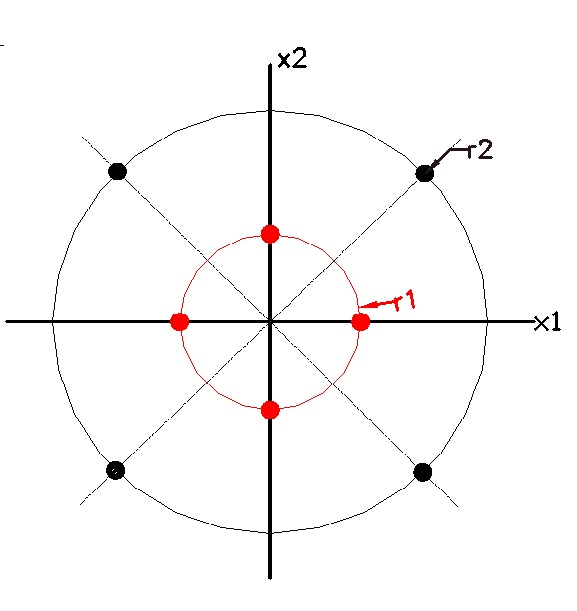
\includegraphics[width=0.15\textwidth]{4thmoment2d1}
      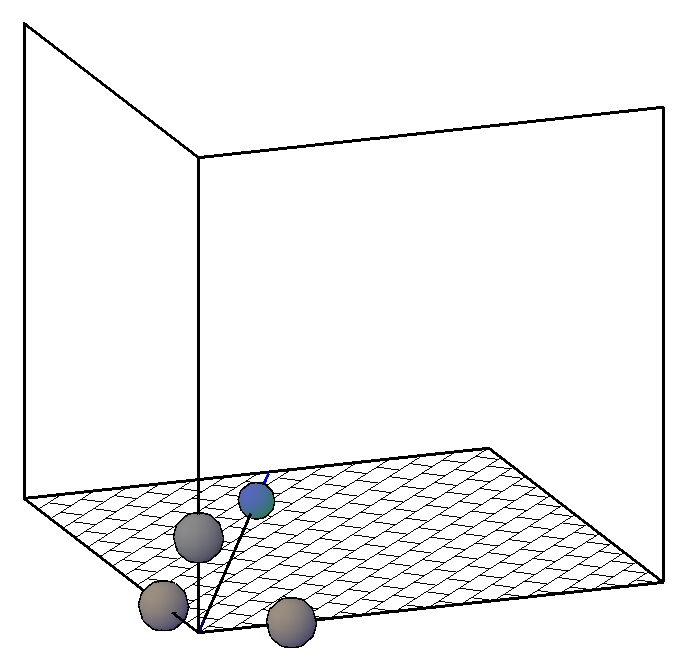
\includegraphics[width=0.15\textwidth]{4thmoment3d1}
      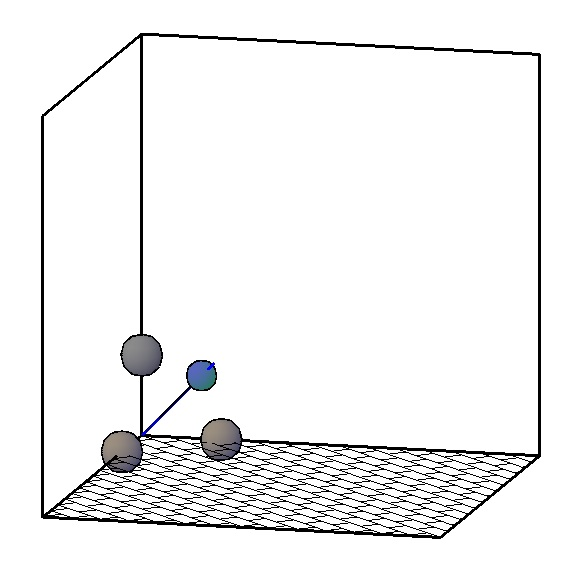
\includegraphics[width=0.15\textwidth]{4thmoment3d3}
      \caption{2D and 3D Cubature points to satisfy 4th order moments}
      \label{fig:23d4m1}
   \end{figure}
The total number of cubature points involved for $n>2$ are $2N+2^N$. 


\subsection{Sigma points that are $6^{th}$ order equivalent}

This section describes a similar process to capture all the moments till $6^{th}$ order till dimension 7. The set of moment constraint equations that are to be solved to get the cubature points and weights is generalised till the $7^{th}$ dimension. As in the procedure followed to capture the $4^{th}$ order moments, firstly the moments till $6^{th}$ order for a continuous PDF are evaluated, secondly the axis are chosen on which the points are to be constrained. Then all the points are enumerated as a set and substituted into the moment constraint equations. The points on the principle axis have each a weight of $w_1$ and are at a distane of $r_1$ from the origin. The points on the $N^th$-Conjugate axis have each a weight of $w_2$ and are located at a distance of $r_2$ along this axis. The third set of points have weight $w_3$ and are located at a distance of $r_3$ along the $2^{nd}$-Conjugate axis. The moments for the continuous normal PDF are    
\setlength{\arraycolsep}{0.0em}
\begin{eqnarray}
&E[X_i^2]=1,\, E[X_iX_j]=0, \, E[X_i^4]=3, \, E[X_i^3X_j]=0 \nonumber\\
&E[X_i^2X_j^2]=1, \, E[X_i^2X_jX_k]=0,\, E[X_iX_jX_kX_l]=0, \, E[X_i^6]=15\nonumber\\
&E[X_i^5X_j]=0 \, E[X_i^4X_j^2]=3,\, E[X_i^4X_jX_k]=0, \, E[X_i^3X_j^3]=0\nonumber\\
&E[X_i^3X_j^2X_k]=0, \, E[X_i^3X_j^2]=0,\,E[X_i^2X_j^2X_k^2]=1 \nonumber\\
&E[X_iX_jX_kX_lX_mX_n]=0\label{6thmoms}
\end{eqnarray}
\setlength{\arraycolsep}{5pt}
As the points chosen are fully symmetric only the moment with all even powers are to be satisfied. The general set of moment constraint equations is\newline
For $N<8$
\setlength{\arraycolsep}{0.0em}
\begin{eqnarray}
2r_1^2w_1+2^Nr_2^2w_2+4(N-1)r_3^2w_3=1\\
2r_1^4w_1+2^Nr_2^4w_2+4(N-1)r_3^4w_3=3\\
2^Nr_2^4w_2+4r_3^4=1\\
2r_1^6w_1+2^Nr_2^6w_2+4(N-1)r_3^6w_3=15\\
2^Nr_2^6w_2+4r_3^6=3\\
2^Nr_2^6w_2=1
\end{eqnarray}
\setlength{\arraycolsep}{5pt}
Solving the last 3 equations ...  for the weights analytically , shows that
 \setlength{\arraycolsep}{0.0em}
\begin{eqnarray}
w_1=\frac{8-n}{r_1^6}\\
w_2=\frac{1}{2^nr_2^6}\\
w_3=\frac{1}{2r_3^6}
\end{eqnarray}
\setlength{\arraycolsep}{5pt}
above dimension 7 one weight starts to become negative. One way to overcome this is to select a new set of axis and repeat the procedure. Once the weigths are symbolically solved from the last 3 equatiosn they can be substituted into the first 3 equations. Then there are only 3 polynomial equations in terms of $r_1$,$r_2$ and $r_3$. This reduced system of equations is much easier to solve than the original system of equations. The points are shown in Fig: 

   \begin{figure}[thpb]
      \centering
      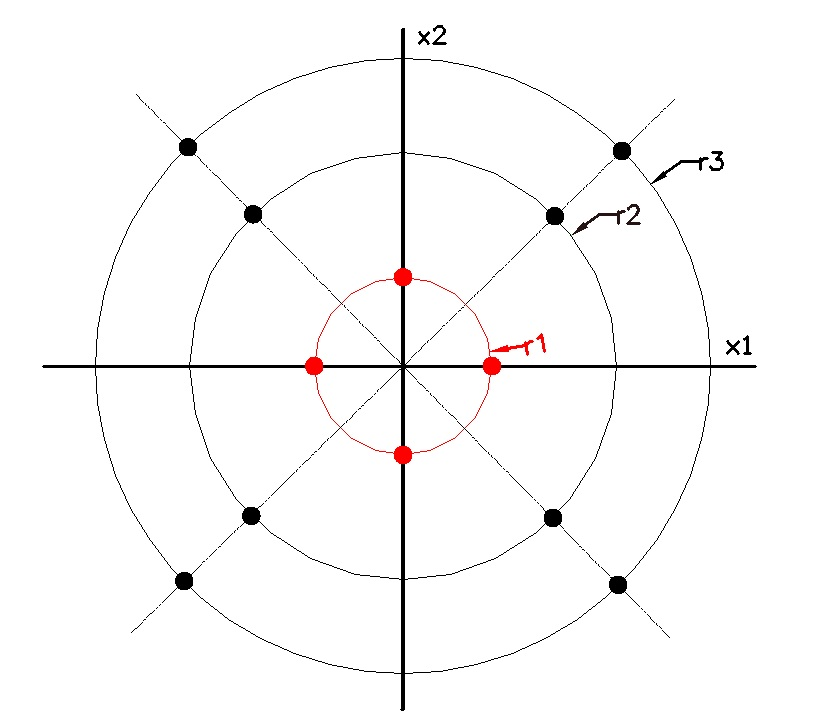
\includegraphics[width=0.15\textwidth]{6thmoment2d1}
      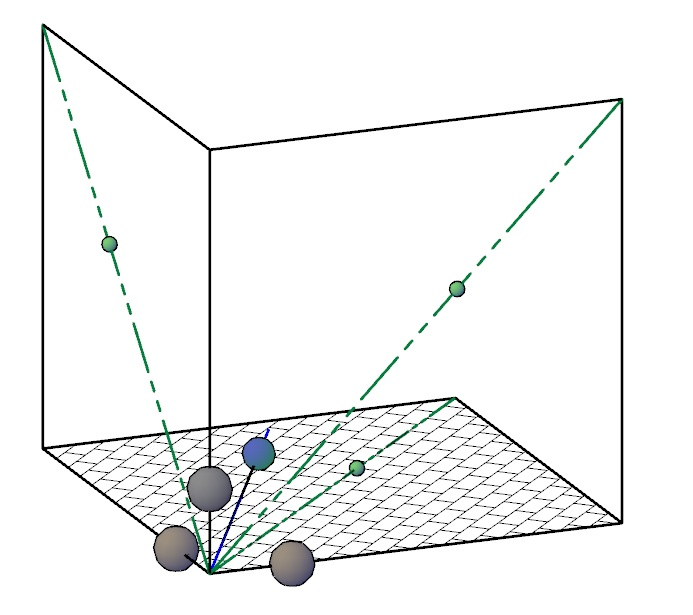
\includegraphics[width=0.15\textwidth]{3d6thmom}
      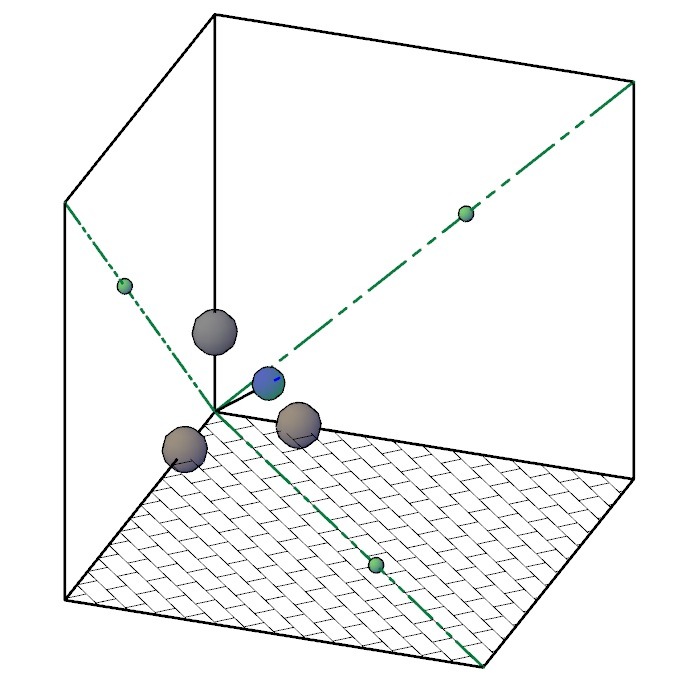
\includegraphics[width=0.15\textwidth]{3d6thmom2}
      \caption{2D and 3D Cubature points to satisfy 6th order moments}
      \label{fig:23d4m1}
   \end{figure}
The total number of cubature points involved in this method to capture all the moments till 6th order is $2N^2+2^N+1$. 

\subsection{Cubature points that are $8^{th}$ order equivalent}
This section describes an attempt to capture all moments equal to and less than 8. 

\section{Results}
This section illustrates various examples using the methods mentioned in this paper. 

%%%%%%%%%%%%%%%%%%%%%%%%%%%%%%%%%%%%%%%%%%%%%%
\subsection{Polynomial nonlinearity}
All the methods are compared against the Gauss Hermite Product rule for multidimensional integral as it is known to exactly integrate polynomials.In general for a polynomial of degree $2m+1$ the Gauss Hermite Product rule for $N^th$-Dimensional integral requires $(m+1)^N$ cubature points. In every case the integral that is being evaluated in the domian $(-\infty,\infty)$ is of the form
\begin{equation}
\mu=E[f(X)]=\int{\int{...\int{f(X)N(X,0|P)}}}dX_1dX_2...dX_N
\end{equation}
where $X=[X_1,X_2,...,X_N]^T$ and $f:R^N \rightarrow R$ i.e. f is a continuous scalar valued polynomial function and R is the set of real numbers. The gaussian weighting function has mean ${\bf 0}$ and covariance matrix as $P$ of appropriate dimensions \newline

%%%%%%%%%%             3          %%%%%%%%%%%%

\subsubsection{Polynomials of degree 3 or less}
For polynomials of degree 3 or less, the Gauss Hermite Product rule would need at least $2^N$ cubature points. The true value of the integral is generated with $5^N$ points and the relative error for each method is compared to this true value. The covariance of the gaussian weighting function is taken to be $P=100I_{NxN}$. This covariance is selected to magnify any error in the cubature points of each method. An example function $f(X)$ for a 4D system with degree 2 is 

\setlength{\arraycolsep}{0.0em}
\begin{eqnarray}
f(X)=\sum_{i=1}^4{X_i^2}+\sum_{i=1}^3{\sum_{j=i+1}^4{X_iX_j}}
\end{eqnarray}
\setlength{\arraycolsep}{5pt}

\begin{table*}
\caption{Comparison for $N=4$ and $2^{nd}$-moment equivalent}
\label{comppoly2int}
\begin{center}
\begin{tabular}{|c||c|c|c|}
\hline
method     & 			n   		 	 	&				$\mu$ 				& \% rel. error						\\
\hline
$GH$   		 &  	 	$ $ 			 	&	  		$	$ 				 	&     $$									 \\
\hline
$UT$ 		   & 			$ $  				&  			$ $ 					& 													\\
\hline 
$CKF$ 		 & 			$ $  				&  			$ $  					&														\\
\hline
$CUT4$ 		 &	  	$ $  				&  			$ $ 					& 													\\
\hline
$CUT6$ 		 & 			$ $  				&  			$	$  					&														\\
\hline
$CUT8$ 		 & 			$ $  				&  			$	$  					&														\\
\hline
\end{tabular}
\end{center}
\end{table*}

%%%%%%%%%%             4          %%%%%%%%%%%%

\subsubsection{Polynomials of degree 5 or less}
For polynomials of degree 5 or less, the Gauss Hermite Product rule would need at least $3^N$ cubature points. The true value of the integral is generated with $7^N$ points and the relative error for each method is compared to this true value. The covariance used is $P=100I_{NxN}$. An example function $f(X)$ for a 4D system with degree 4 and all even powers is 

\setlength{\arraycolsep}{0.0em}
\begin{eqnarray}
f(X)=\sum_{i=1}^4{X_i^4}+\sum_{i=1}^4{X_i^2}+\sum_{i=1}^3{\sum_{j=i+1}^4{X_i^2X_j^2}}
\end{eqnarray}
\setlength{\arraycolsep}{5pt}


%%%%%%%%%%             6          %%%%%%%%%%%%

\subsubsection{Polynomials of degree 7 or less}
For polynomials of degree 7 or less, the Gauss Hermite Product rule would need at least $4^N$ cubature points. The true value of the integral is generated with $9^N$ points and the relative error for each method is compared to this true value. The covariance used is $P=100I_{NxN}$. An example function $f(X)$ for a 5D system with degree 6 and all even powers is 

\setlength{\arraycolsep}{0.0em}
\begin{eqnarray}
f(X)=\sum_{i=1}^5{X_i^6}+\sum_{i=1}^5{X_i^4}+\sum_{i=1}^5{X_i^2}+\sum_{i=1}^4{\sum_{j=i+1}^5{X_i^2X_j^2}}\\
+\sum_{i=1}^4{\sum_{j=i+1}^5{X_i^4X_j^2}}+\sum_{i=1}^4{\sum_{j=i+1}^3{\sum_{k=j+1}^2{X_i^2X_j^2}}}
\end{eqnarray}
\setlength{\arraycolsep}{5pt}

\begin{table*}
\caption{Comparison for $N=5$ and $6^{th}$-moment equivalent}
\label{comppoly4int}
\begin{center}
\comments{
\begin{tabular}{|c||c|c|c|}
\hline
method     & 			n   		 	 	&				$\mu$ 				& \% rel. error						\\
\hline
$GH$   		 &  	 	$ $ 			 	&	  		$	$ 				 	&     $$									 \\
\hline
$UT$ 		   & 			$ $  				&  			$ $ 					& 													\\
\hline 
$CKF$ 		 & 			$ $  				&  			$ $  					&														\\
\hline
$CUT4$ 		 &	  	$ $  				&  			$ $ 					& 													\\
\hline
$CUT6$ 		 & 			$ $  				&  			$	$  					&														\\
\hline
$CUT8$ 		 & 			$ $  				&  			$	$  					&														\\
\hline
\end{tabular}
}
\begin{tabular}{|c||c|c|c|}
\hline
method     & 			n   		 	 	&				$\mu$ 				& \% rel. error						\\
\hline
$GH$   		 &  	 	$ $ 			 	&	  		$	$ 				 	&     $$									 \\
\hline
$UT$ 		   & 			$ $  				&  			$ $ 					& 													\\
\hline 
$CKF$ 		 & 			$ $  				&  			$ $  					&														\\
\hline
$CUT4$ 		 &	  	$ $  				&  			$ $ 					& 													\\
\hline
$CUT6$ 		 & 			$ $  				&  			$	$  					&														\\
\hline
$CUT8$ 		 & 			$ $  				&  			$	$  					&														\\
\hline
\end{tabular}
%\end{center}
%\begin{center}
\begin{tabular}{|c||c|c|c|}
\hline
method     & 			n   		 	 	&				$\mu$ 				& \% rel. error						\\
\hline
$GH$   		 &  	 	$ $ 			 	&	  		$	$ 				 	&     $$									 \\
\hline
$UT$ 		   & 			$ $  				&  			$ $ 					& 													\\
\hline 
$CKF$ 		 & 			$ $  				&  			$ $  					&														\\
\hline
$CUT4$ 		 &	  	$ $  				&  			$ $ 					& 													\\
\hline
$CUT6$ 		 & 			$ $  				&  			$	$  					&														\\
\hline
$CUT8$ 		 & 			$ $  				&  			$	$  					&														\\
\hline
\end{tabular}
\begin{tabular}{|c||c|c|c|}
\hline
method     & 			n   		 	 	&				$\mu$ 				& \% rel. error						\\
\hline
$GH$   		 &  	 	$ $ 			 	&	  		$	$ 				 	&     $$									 \\
\hline
$UT$ 		   & 			$ $  				&  			$ $ 					& 													\\
\hline 
$CKF$ 		 & 			$ $  				&  			$ $  					&														\\
\hline
$CUT4$ 		 &	  	$ $  				&  			$ $ 					& 													\\
\hline
$CUT6$ 		 & 			$ $  				&  			$	$  					&														\\
\hline
$CUT8$ 		 & 			$ $  				&  			$	$  					&														\\
\hline
\end{tabular}
\end{center}
\end{table*}

%%%%%%%%%%             8          %%%%%%%%%%%%

\subsubsection{Polynomials of degree 9 or less}
For polynomials of degree 5 or less, the Gauss Hermite Product rule would need at least $3^N$ cubature points. The true value of the integral is generated with $7^N$ points and the relative error for each method is compared to this true value. The covariance used is $P=100I_{NxN}$. An example function $f(X)$ for a 5D system with degree 4 and all even powers is 

\setlength{\arraycolsep}{0.0em}
\begin{eqnarray}
f(X)=\sum_{i=1}^5{X_i^4}+\sum_{i=1}^5{X_i^2}+\sum_{i=1}^4{\sum_{j=i+1}^5{X_i^2X_j^2}}
\end{eqnarray}
\setlength{\arraycolsep}{5pt}
%%%%%%%%%%%%%%%%%%%%%%%%%%%%
%%%%%%%%%%%%%%%%%%%%%%%%%%%%%%%%%%%%%%%%%%%%%%



\subsection{Non-polynomial nonlinearity}

\subsubsection{Polar to Cartesian coordinates}
The example in ref...all the methods seem to do well
   \begin{figure}[thpb]
      \centering
      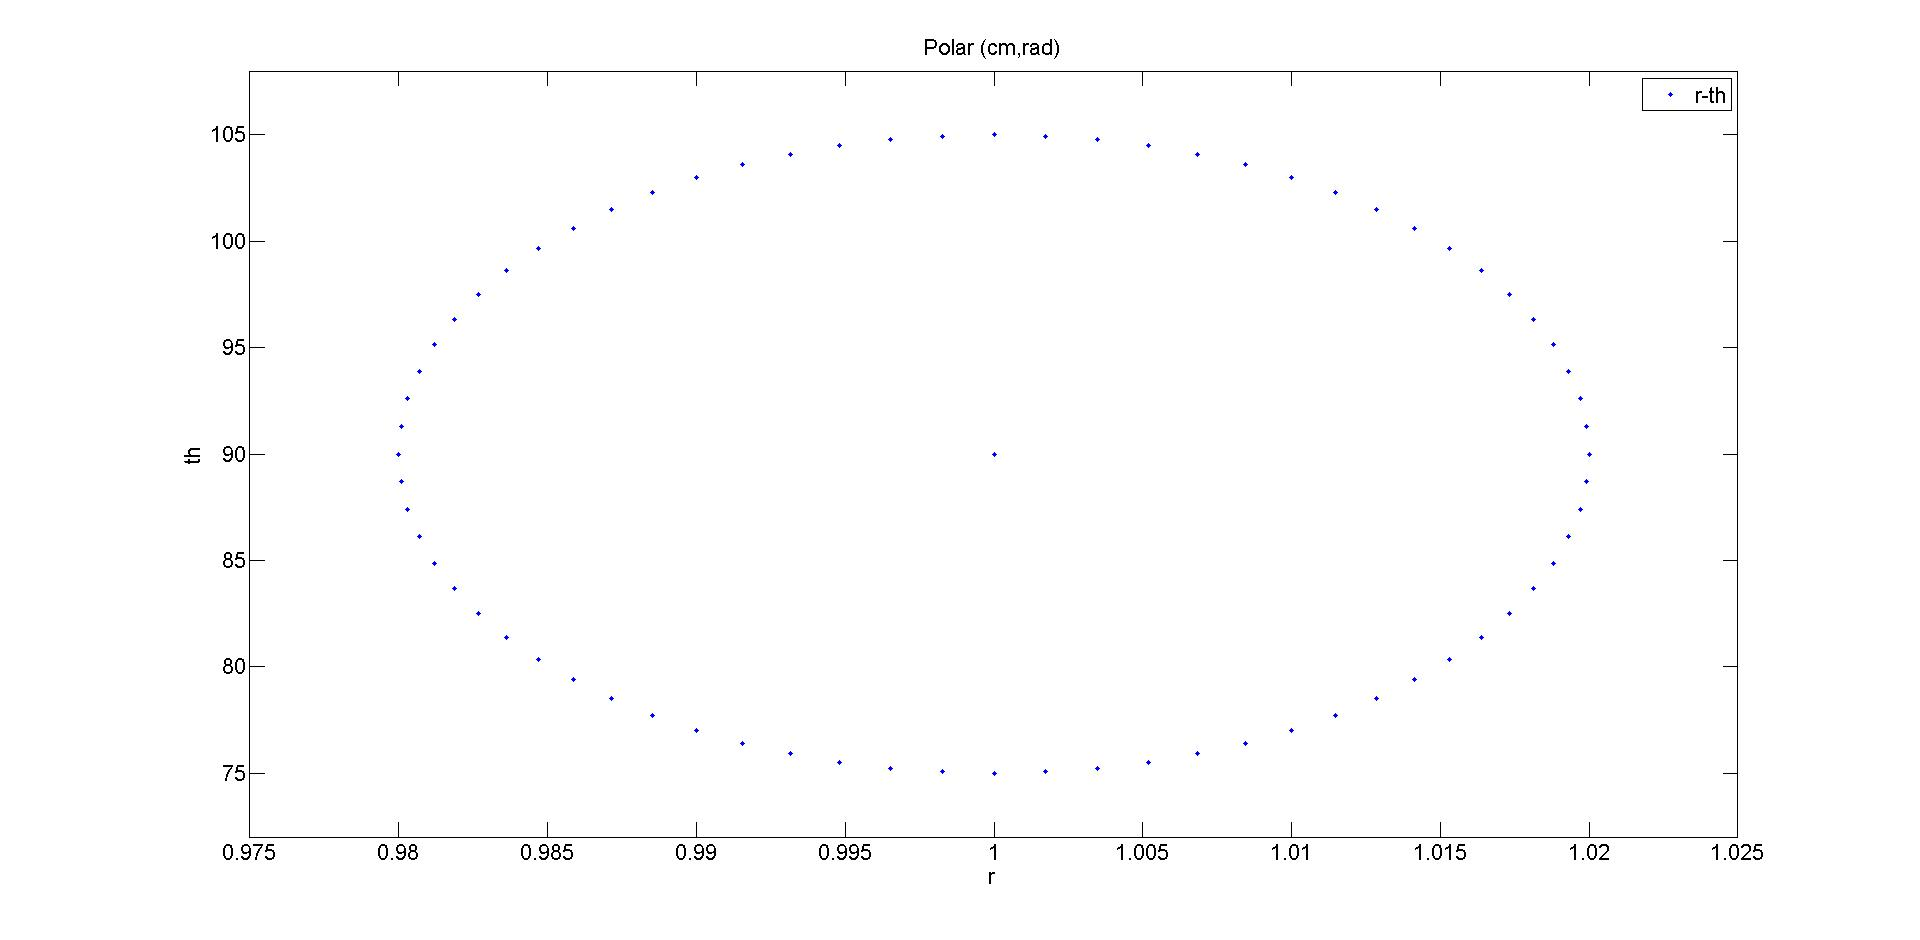
\includegraphics[width=0.2\textwidth]{polartocart5}
      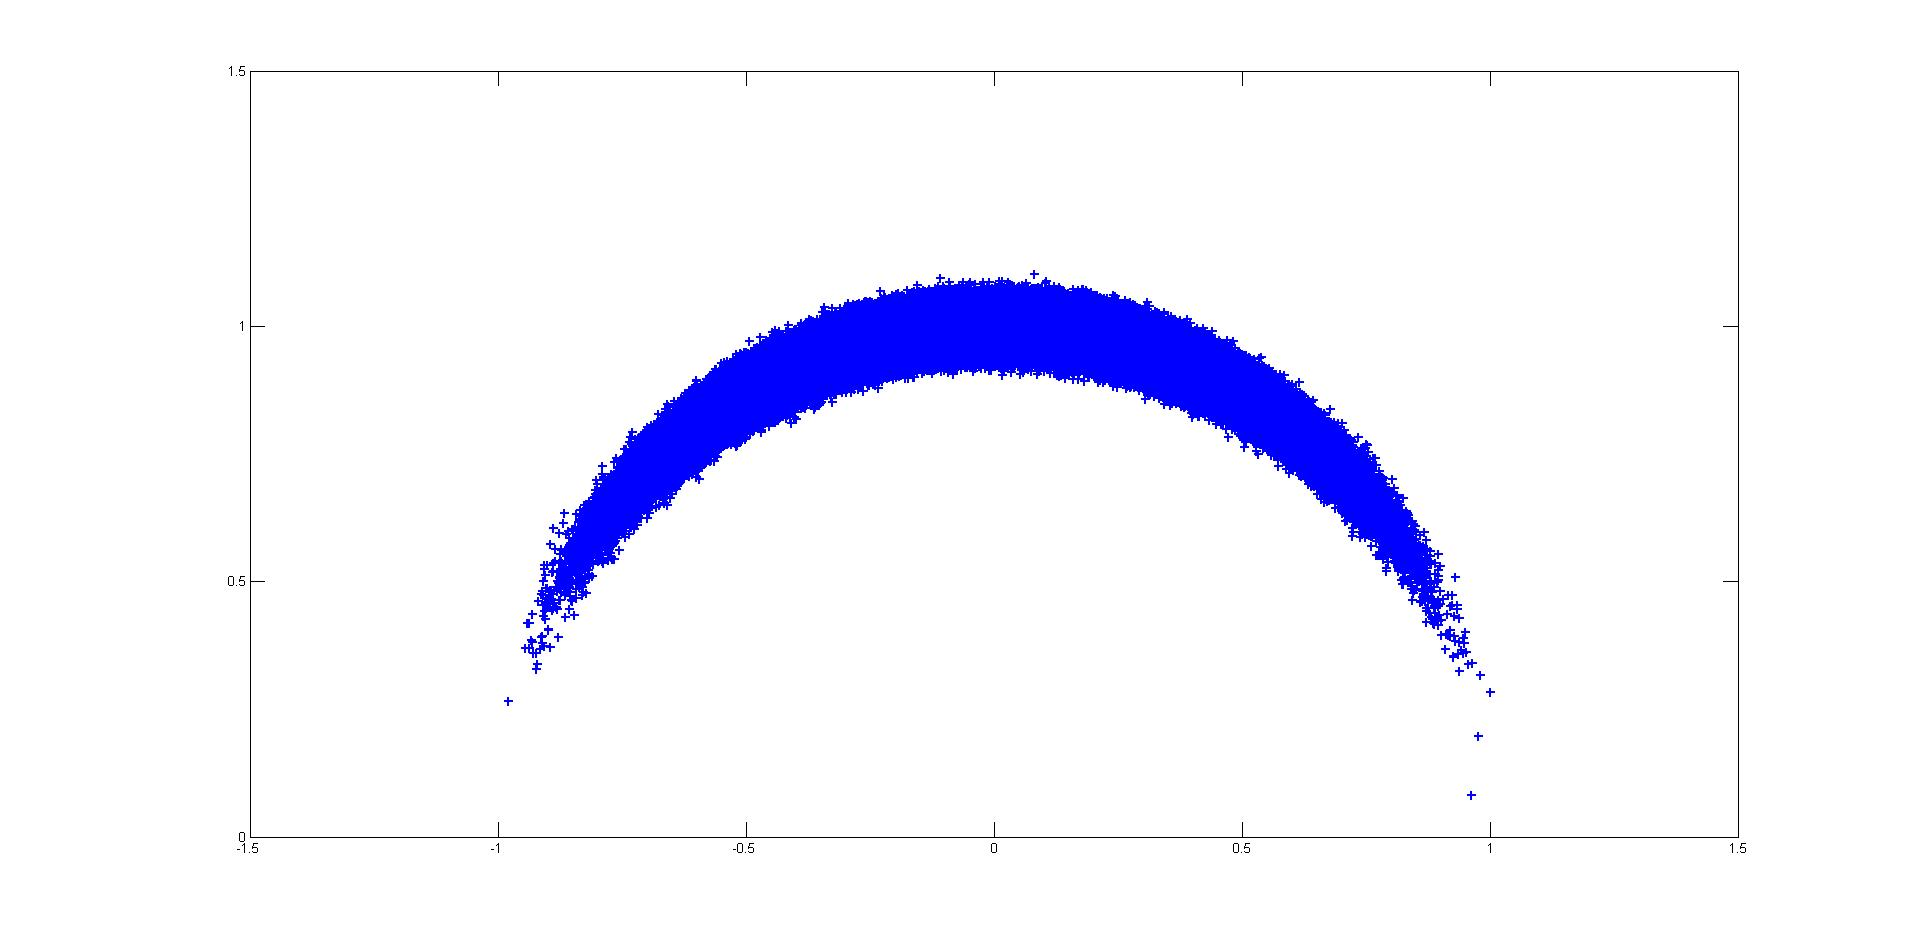
\includegraphics[width=0.2\textwidth]{polartocart4}
      \caption{2D and 3D Cubature points to satisfy 6th order moments}
      \label{fig:23d4m1}
   \end{figure}
      \begin{figure}[thpb]
      \centering
      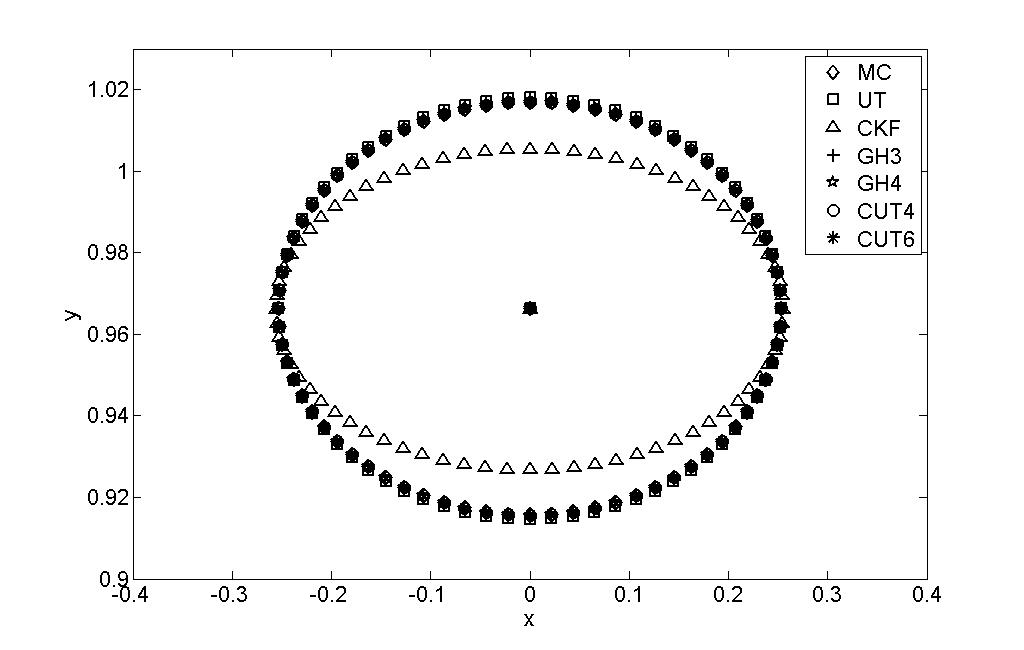
\includegraphics[width=0.5\textwidth]{polartocart3}
      \caption{2D and 3D Cubature points to satisfy 6th order moments}
      \label{fig:23d4m1}
   \end{figure}  
For the same example when the covariance for radial direction is increased the higher moment methods seem to do better
   
   \begin{figure}[thpb]
      \centering
      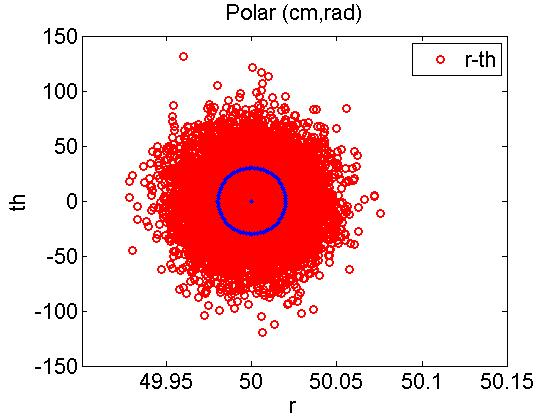
\includegraphics[width=0.2\textwidth]{polar}
      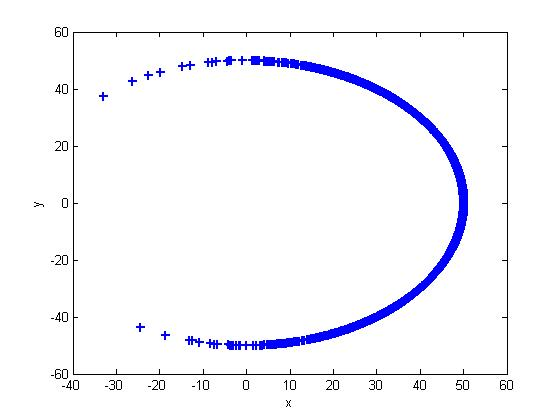
\includegraphics[width=0.2\textwidth]{polartocart2}
      \caption{2D and 3D Cubature points to satisfy 6th order moments}
      \label{fig:23d4m1}
   \end{figure} 
   
   \begin{figure}[thpb]
      \centering
      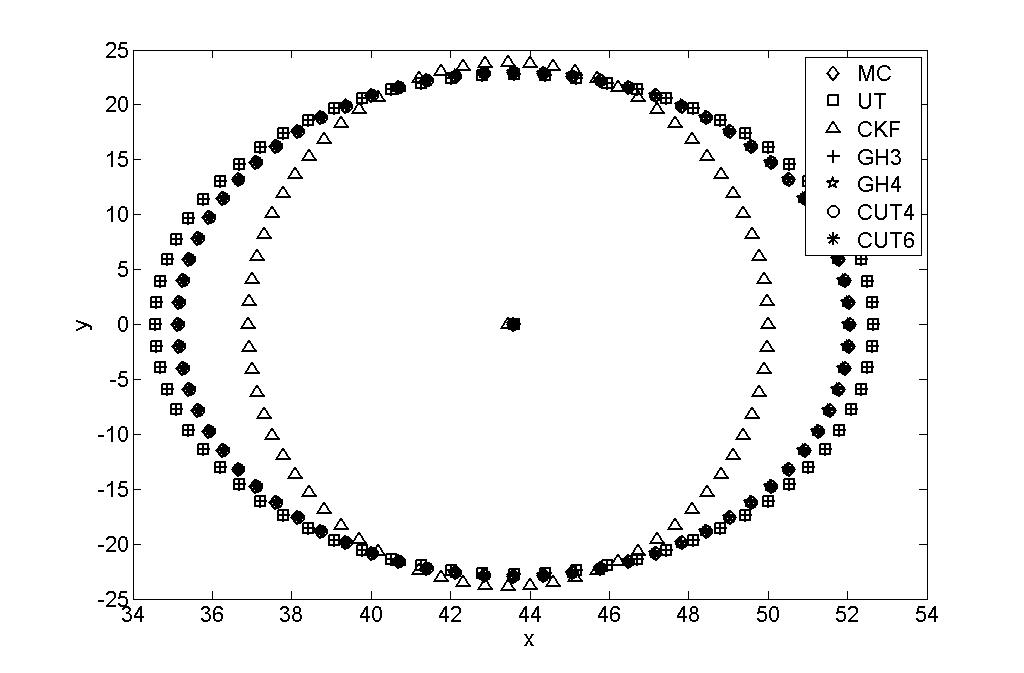
\includegraphics[width=0.5\textwidth]{polartocart}
      \caption{2D and 3D Cubature points to satisfy 6th order moments}
      \label{fig:23d4m1}
   \end{figure} 

%%%%%%%%%%%%%%%%%%%%%%%%%%
\subsubsection{Exponential functions}

\subsubsection{CKF example}


\addtolength{\textheight}{-3cm}   % This command serves to balance the column lengths
                                  % on the last page of the document manually. It shortens
                                  % the textheight of the last page by a suitable amount.
                                  % This command does not take effect until the next page
                                  % so it should come on the page before the last. Make
                                  % sure that you do not shorten the textheight too much.

%%%%%%%%%%%%%%%%%%%%%%%%%%%%%%%%%%%%%%%%%%%%%%%%%%%%%%%%%%%%%%%%%%%%%%%%%%%%%%%%

%%%%%%%%%%%%%%%%%%%%%%%%%%%%%%%%%%%%%%%%%%%%%%%%%%%%%%%%%%%%%%%%%%%%%%%%%%%%%%%%
\section{DISCUSSIONS and CONCLUSIONS}

\subsection{Discussion about the Pros and Cons}

\subsection{Conclusion}

%%%%%%%%%%%%%%%%%%%%%%%%%%%%%%%%%%%%%%%%%%%%%%%%%%%%%%%%%%%%%%%%%%%%%%%%%%%%%%%%
\section{ACKNOWLEDGMENTS}



%%%%%%%%%%%%%%%%%%%%%%%%%%%%%%%%%%%%%%%%%%%%%%%%%%%%%%%%%%%%%%%%%%%%%%%%%%%%%%%%
\begin{thebibliography}{99}

\bibitem{c1}
J.G.F. Francis, The QR Transformation I, {\it Comput. J.}, vol. 4, 1961, pp 265-271.

\bibitem{c2}
H. Kwakernaak and R. Sivan, {\it Modern Signals and Systems}, Prentice Hall, Englewood Cliffs, NJ; 1991.

\bibitem{c3}
D. Boley and R. Maier, "A Parallel QR Algorithm for the Non-Symmetric Eigenvalue Algorithm", {\it in Third SIAM Conference on Applied Linear Algebra}, Madison, WI, 1988, pp. A20.

\end{thebibliography}

\end{document}
